\backmatter
%Formato de página sin header ni raya arriba
\renewcommand\headrulewidth{0pt}
\pagestyle{empty}
  \fancyhf{}
\fancypagestyle{plain}{}
\fancypagestyle{fancy}{}
\printindex{}

%\begin{center}
%{\Huge A BOOK}
%Cómo usar Google Earth Engine y no fallar en el intento, editado por el Centro de Investigaciones en Geografía Ambiental y el Instituto de Investigación de Recursos Biológicos Alexander von Humboldt se publicó el [dd] de agosto de 2022. Para su formación se utilizaron las tipografías Latin Modern Roman y Computer Modern Roman en 12, 15, 17 y 21 pt. El cuidado de la edición estuvo al cuidado de Jonathan Vidal Solórzano Villegas, Gabriel Alejandro Perilla Suárez, Mónica Braun y Jorge Andrés Trinidad González. El diseño editorial estuvo a cargo de Jonathan Vidal Solórzano Villegas y Laura Perilla Suárez.
%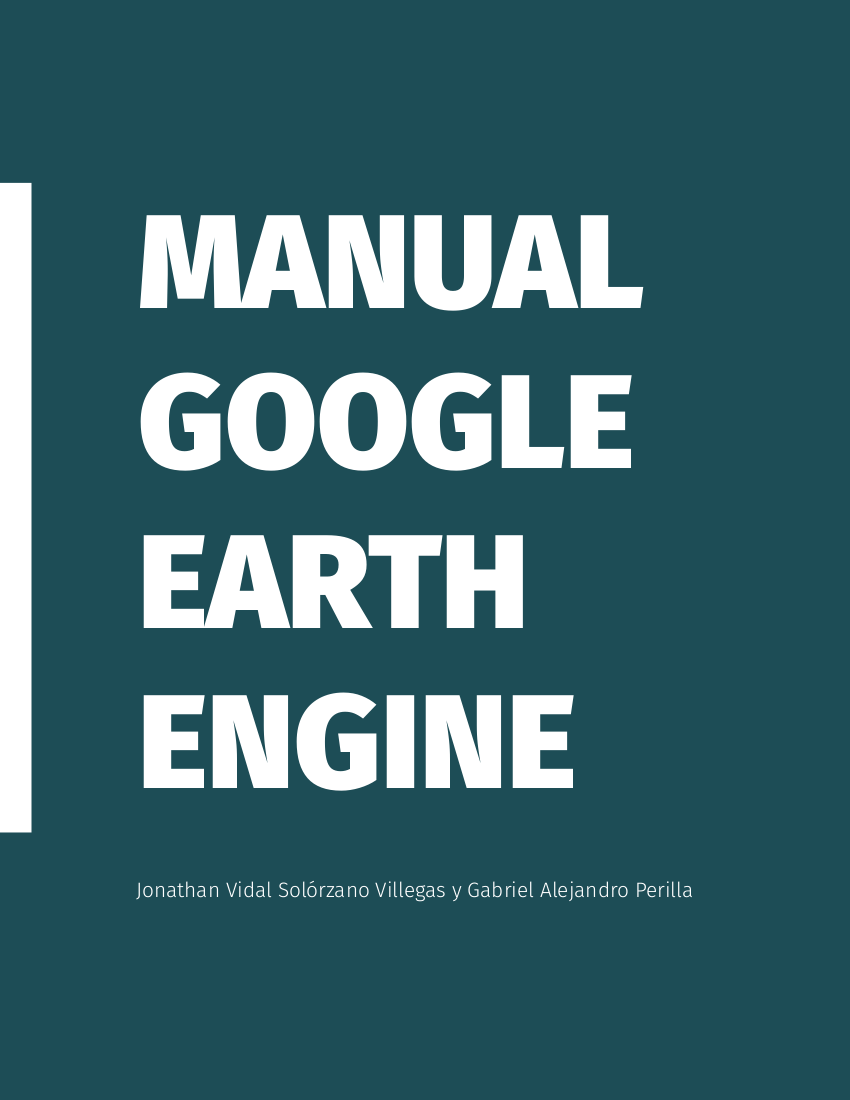
\includegraphics{Img/Portada.png}
%{\huge by Jonathan Vidal Solórzano Villegas y Alejandro Perilla Suárez}
%\end{center}